\section{Overview: The Cinderella-Stepmother Game}
\label{sec:example}

We illustrate the flow of the validity guided-synthesis algorithm using a variation of the minimum-backlog
problem, the two player game between Cinderella and her wicked Stepmother, first expressed by Bodlaender \textit{et al.}~\cite{bodlaender2012cinderella}.

The main objective for Cinderella (i.e. the reactive system) is to prevent a
collection of buckets from overflowing with water. On the other hand,
Cinderella's Stepmother (i.e. the system's environment) refills the buckets with a predefined amount of water that is distributed in a random fashion between the buckets.
For the running example, we chose an instance of the game that has been
previously used in template-based synthesis~\cite{beyene2014constraint}. In this instance, the game is described
using five buckets, where each bucket can contain up to two units of water.
Cinderella has the option to empty two adjacent buckets at each of her turns,
while the Stepmother distributes one unit of water over all five buckets. In the context of this paper we use this example to show how specification is expressed, as well as how we can synthesize an efficient implementation that describes reactions for Cinderella, such that a bucket overflow is always prevented.

\begin{figure}[!t]
\centering
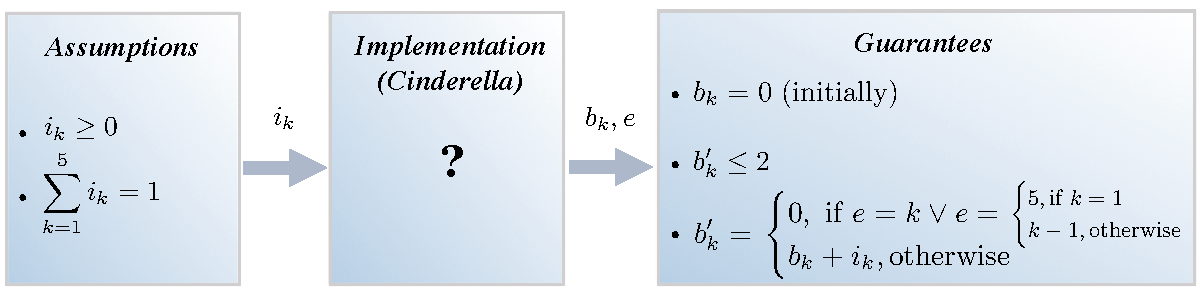
\includegraphics[scale=0.6]{agcontract.pdf}
\caption{An Assume-Guarantee contract.}
\label{fg:agcontract}
\end{figure}

We represent the system requirements using an \textit{Assume-Guarantee
Contract}. The \emph{assumptions} of the contract restrict the possible inputs that the
environment can provide to the system, while the \emph{guarantees}
describe safe reactions of the system to the outside world.

A (conceptually) simple example is shown in Fig.~\ref{fg:agcontract}. The contract describes a possible set of requirements for a specific instance of the Cinderella-Stepmother game. % that we introduced in Sect.~\ref{sec:example}.
Our goal is to synthesize an implementation that describes Cinderella's winning region of the game. Cinderella in this case is the implementation, as shown by the middle box in Fig.~\ref{fg:agcontract}. Cinderella's inputs are five different values $i_k$, $1 \leq k \leq 5$, determined by a random distribution of one unit of water by the Stepmother. During each of her turns Cinderella has to make a choice denoted by the output variable $e$, such that the buckets $b_k$ do not overflow during the next action of her Stepmother. We define the contract using the set of assumptions $A$ (left box in Fig.~\ref{fg:agcontract}) and the guarantee constraints $G$ (right box in Fig.~\ref{fg:agcontract}). For the particular example, it is possible to construct at least one implementation that satisfies $G$ given $A$ which is described in Sect.~\ref{sec:algexample}.
The proof of existence of such an implementation is the main concept behind the \emph{realizability} problem, while the automated construction of a witness implementation is the main focus of \emph{program synthesis}.

Given a proof of realizability of the contract in Fig.~\ref{fg:agcontract}, % is \emph{realizable}, there should exist at least one implementation, and 
we are seeking for an efficient synthesis procedure that could provide an implementation.
On the other hand, consider a variation of the example, where $A = \mathit{true}$. This is a practical case of an
\emph{unrealizable} contract, as there is no feasible Cinderella implementation that can correctly react to Stepmother's actions. An example counterexample allows the Stepmother to pour random amounts of water into the buckets, leading to overflow of at least one bucket during each of her turns.

\section{Background}
\label{sec:background}
%\label{sec:formals}
We use two disjoint sets, $state$ and $inputs$, to describe a system.
A straightforward and intuitive way to represent an \emph{implementation} is by
defining a \emph{transition system}, composed of an initial state
predicate $I(s)$ of type $state \to bool$, as well as a transition relation
$T(s,i,s')$ of type $state \to inputs \to state \to bool$.

Combining the above, we represent an Assume-Guarantee (AG) contract using a set
of \emph{assumptions}, $A: state \rightarrow inputs \rightarrow bool$,
and a set of \emph{guarantees} $G$. The latter is further decomposed into two
distinct subsets $G_I: state \rightarrow bool$ and $G_T: state \rightarrow
inputs \rightarrow state \rightarrow bool$. The $G_I$ defines the set of valid
initial states, and $G_T$ contains constraints that need to be satisfied in
every transition between two states. Importantly, we
do not make any distinction between the internal state variables and the output variables in the
formalism. This allows us to use the state variables to (in some cases)
simplify the specification of guarantees since a contract
might not be always defined over all variables in the transition system.

Consequently, we can formally define a realizable contract, as one for which any
preceding state $s$ can  transition into a new state $s'$ that satisfies
the guarantees, assuming valid inputs. For a system to be ever-reactive, these
new states $s'$ should be further usable as preceding states in a future
transition. States like $s$ and $s'$ are called \textit{viable} if
and only if:
\begin{align}
\begin{split}
  \viable(s) &=
  \forall i. (A(s, i) \Rightarrow \exists s'.~ G_T(s, i,s')
\land \viable(s'))
\label{eq:viable}
\end{split}
\end{align}
This equation is recursive and we interpret it coinductively, i.e., as a
greatest fixpoint.
A necessary condition, finally, is that the intersection of sets of viable states
and initial states is non-empty. As such, to conclude that a contract
is realizable, we require that
\begin{equation}
\exists s. G_I(s) \land \viable(s)
\label{eq:nonempty}
\end{equation}

\noindent The synthesis problem is therefore to determine an initial state $s_i$ and function $f(s, i)$ such that $G_I(s_i)$ and $\forall s, i . \viable(s) \Rightarrow \viable(f(s, i))$.

The intuition behind our proposed algorithm in this paper relies on the
discovery of a fixpoint $F$ that only contains viable states.  We can determine whether $F$ is a fixpoint by proving the validity of the following formula:
\[
\forall s,i. \ (F(s) \land A(s,i) \Rightarrow \exists s'.G_{T}(s,i,s') \land F(s'))
\]

\noindent In the case where the greatest fixpoint $F$ is non-empty, we check whether it satisfies $G_{I}$ for some initial state.  If so, we proceed by extracting a witnessing initial state and witnessing skolem function $f(s, i)$ to determine $s'$ that is, by construction, guaranteed to satisfy the specification.

To achieve both the fixpoint generation and the witness extraction, we depend on \aeval, a solver for $\forall\exists$-formulas.

\subsection{Skolem functions and regions of validity}
\label{sec:aeval}


%\andreas{I believe the section can be a bit longer. I also think that the keyphrase ``region of validity'' needs to stand out more. Finally, a proof for Lemma 1, or at least an outline of it would be greatly appreciated.}

We rely on the already established algorithm to decide the validity of $\forall\exists$-formulas and extract Skolem functions, called \aeval~\cite{fedyukovich2015automated}.
It takes as input a formula $\forall x \,.\, \exists y  \,.\, \Phi (x, y)$ where $\Phi (x, y)$ is quantifier-free.
To decide its validity, \aeval first normalizes $\Phi (x, y)$ to the form $S(x) \Rightarrow T(x, y)$ and then attempts to extend all models of $S(x)$ to models of $T(x,y)$.
If such an extension is possible, then the input formula is valid, and a relationship between $x$ and $y$ are gathered in a Skolem function.
Otherwise the formula is invalid, and no Skolem function exists.
We refer the reader to~\cite{KatisFGBGW16} for more details on the Skolem-function generation.

Our approach presented in this paper relies on the fact that during each run, \aeval iteratively creates a set of formulas $\{P_i(x)\}$, such that each $P_i(x)$ has a common model with $S(x)$ and $P_i(x) \Rightarrow \exists y \,.\,T (x,y)$.
After $n$ iterations, \aeval establishes a formula $R_n(x) \eqdef \bigvee_{i=1}^n P_i(x)$ which by construction implies $\exists y\,.\,T(x,y)$.
If additionally $S(x)\Rightarrow R_n(x)$, the input formula is valid, and the algorithm terminates.
%
Fig.~\ref{fg:aeval} shows a Venn diagram for an example of the opposite scenario: $R_2(x) = T_1(x) \lor T_2(x)$, but the input formula is invalid.
However, models of each $S(x) \land P_i(x)$ can still be extended to a model of $T(x, y)$.
%Models of $S(x) \land \neg{R_2(x)}$ cannot be extended to models of $T(x,y)$, thus no formula $T_3(x)$ exists, and \aeval terminates.
% \john {Because we are are already using $A$ and $G$ to represent meaningful formulas I suggest that we use different symbols here so it is not confusing. Especially because the symbols have different signatures in these locations.}

In general, if after $n$ iterations $S(x) \land T(x,y) \land \neg R_n(x)$ is unsatisfiable,
then \aeval terminates.
Note that the formula $\forall x.~ S(x) \land R_n(x) \Rightarrow \exists y .~T(x,y)$ is valid by construction at any iteration of the algorithm.
%Thus, a Skolem function can be generated for it.
%Intuitively, a Skolem function
%describes how $y$ is computed from $s$ in order to satisfy the
%previous formula.
%
We say that $R_n(x)$ is a \emph{region of validity}, and in this work, we are interested in the \emph{maximal} regions of validity, i.e., the ones produced by disjoining all $\{P_i(x)\}$ produced by \aeval before termination and by conjoining it with $S(x)$.
Throughout the paper, we assume that all regions of validity are maximal.
% \john{It is a bit strange how we alternate using formulas that have no free variables along with formulas whose free variables are meant to be implicitly existentially quantified. I think we should either stick with a notation or explicitly say that free variables are interpreted to be existentially quantified.}

% \begin{lemma}
% If formula $\forall x \,.\,  S(x) \Rightarrow \exists y . T(x,y)$ is invalid, and $R_n(x)$ is the region of validity, then there is no other formula $S(x)$ such that $S(x) \land R_n(x) \Rightarrow S(x)$ and $\forall x \,.\,  S(x) \Rightarrow \exists y . T(x,y)$.
% \label{lem:subset}
% \end{lemma}

% \begin{proof}
% Suppose that $S(x)$ exists.
% Then $S(x) \land \neg{R_n(x)} \land S(x)$ is satisfiable, and its models are not contained in $R_n(x)$.
% It contradicts our assumption that \aeval has terminated since otherwise it would proceed for generating $T_{n+1}(x)$ which in turn would enlarge the region of validity.
% \end{proof}

\begin{figure}[!t]
\centering
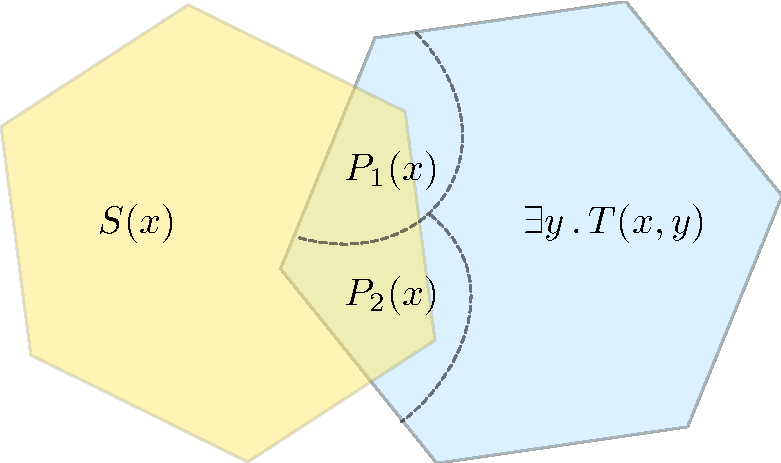
\includegraphics[scale=0.47]{aeval_invalid}
\caption{Region of validity computed for an example requiring \aeval to iterate two times.}
\label{fg:aeval}
\end{figure}

\begin{lemma}\label{lem:aeval}
  Let $R_n(x)$ be the region of validity returned by \aeval for  formula $\forall
  s.~ S(x) \Rightarrow \exists y\,.\,T(x,y)$. Then
%  \begin{equation*}
$  \forall x.~ S(x) \Rightarrow (R_n(x) \Leftrightarrow \exists y\,.\,T(x,y))$.
%  \end{equation*}
\end{lemma}
\begin{proof}
  ($\Rightarrow$) By construction of $R_n(x)$.

  ($\Leftarrow$) Suppose towards contradiction that the formula does
  not hold. Then there exists $x_0$ such that $S(x_0) \land (\exists
  y. T(x_0, y)) \land \neg R_n(x_0)$ holds. But this is a direct
  contradiction for the termination condition for \aeval. Therefore
  the original formula does hold.
\end{proof}

% \begin{corollary}
% If formula $\forall x \,.\,  S(x) \Rightarrow \exists y . T(x,y)$ is invalid, and $R_n(x)$ is the region of validity, then $S(x) \land R_n(x) \Leftrightarrow \exists y . T(x,y)$.
% \label{cor:intermediate}
% \end{corollary}

% \begin{proof}
% ($\Rightarrow$) is immediate from the definition of region of validity.
% ($\Leftarrow$).  Suppose towards contradiction that $s$ satisfies $\exists y . T(x,y)$ but not $S(x) \land R_n(x)$.  If we define $S = s$, we violate Lemma~\ref{lem:subset}.
% \end{proof} 

% \begin{corollary}
% If formula $\forall x \,.\,  S(x) \Rightarrow \exists y . T(x,y)$ is invalid, and $S(x) \land R_n(x)$ is the region of validity, then 
%  $\forall x \,.\, R_n(x) \Leftrightarrow (S(x) \Rightarrow \exists y . T(x,y))$ 
% \label{cor:subset}
% \end{corollary}

% \begin{proof}
% ($\Rightarrow$) Given $s$, suppose $R_n(x)$ is true.  If $S(x)$ is false, then by Corollary~\ref{cor:intermediate},  $\exists y . T(x,y)$ is false, so the implication holds.  Simlarly for $S(x)$ true.
% ($\Leftarrow$) Suppose $S(x) \Rightarrow \exists y . T(x,y)$ is true.  Suppose $S(x)$ is false.  Then $G(s, y)$ might be true and $R_n(x)$ might be false, violating our equivalence.  Boo!
% \end{proof}


